\section{数据收集}
\zihao{-4}
\label{section:data_collection}

FAIR利用Amazon Mechanical Turk进行了两人间多项目谈判的自然语言数据收集任务,共收集了5808个对话数据集。
在本篇论文中,FAIR对于\quotes{两人间多项目谈判}的定义引用于\citet{Fershtman-4,DevaultMell-5},
若不实现阅读这两篇参考文献,读者很容易对谈判产生误解,误解为两位代理需要通过谈判交易对方的资源。
实际上,在该谈判下,项目为两位代理要瓜分的资源,价值为随机生成;
用户即代理仅知道自己的项目价值,另外一个代理的项目价值函数需要通过对话推理得出;
输出为用户通过谈判结果所认为自己所应该得到项目部分。

值得注意的是,
谈判结果可以为成交即\quotes{Deal},也可以为失败即\quotes{No Deal},
那么如何确定谈判结果的标的?
如项目和输出的定义,若谈判成交,则两位用户输出的各项目之和应当分别等于各项目总数。
因此,FAIR在本文中以\quotes{输出的各项目之和应当分别等于各项目总数}作为谈判结果的标的。

\begin{figure*}[ht]
\centering
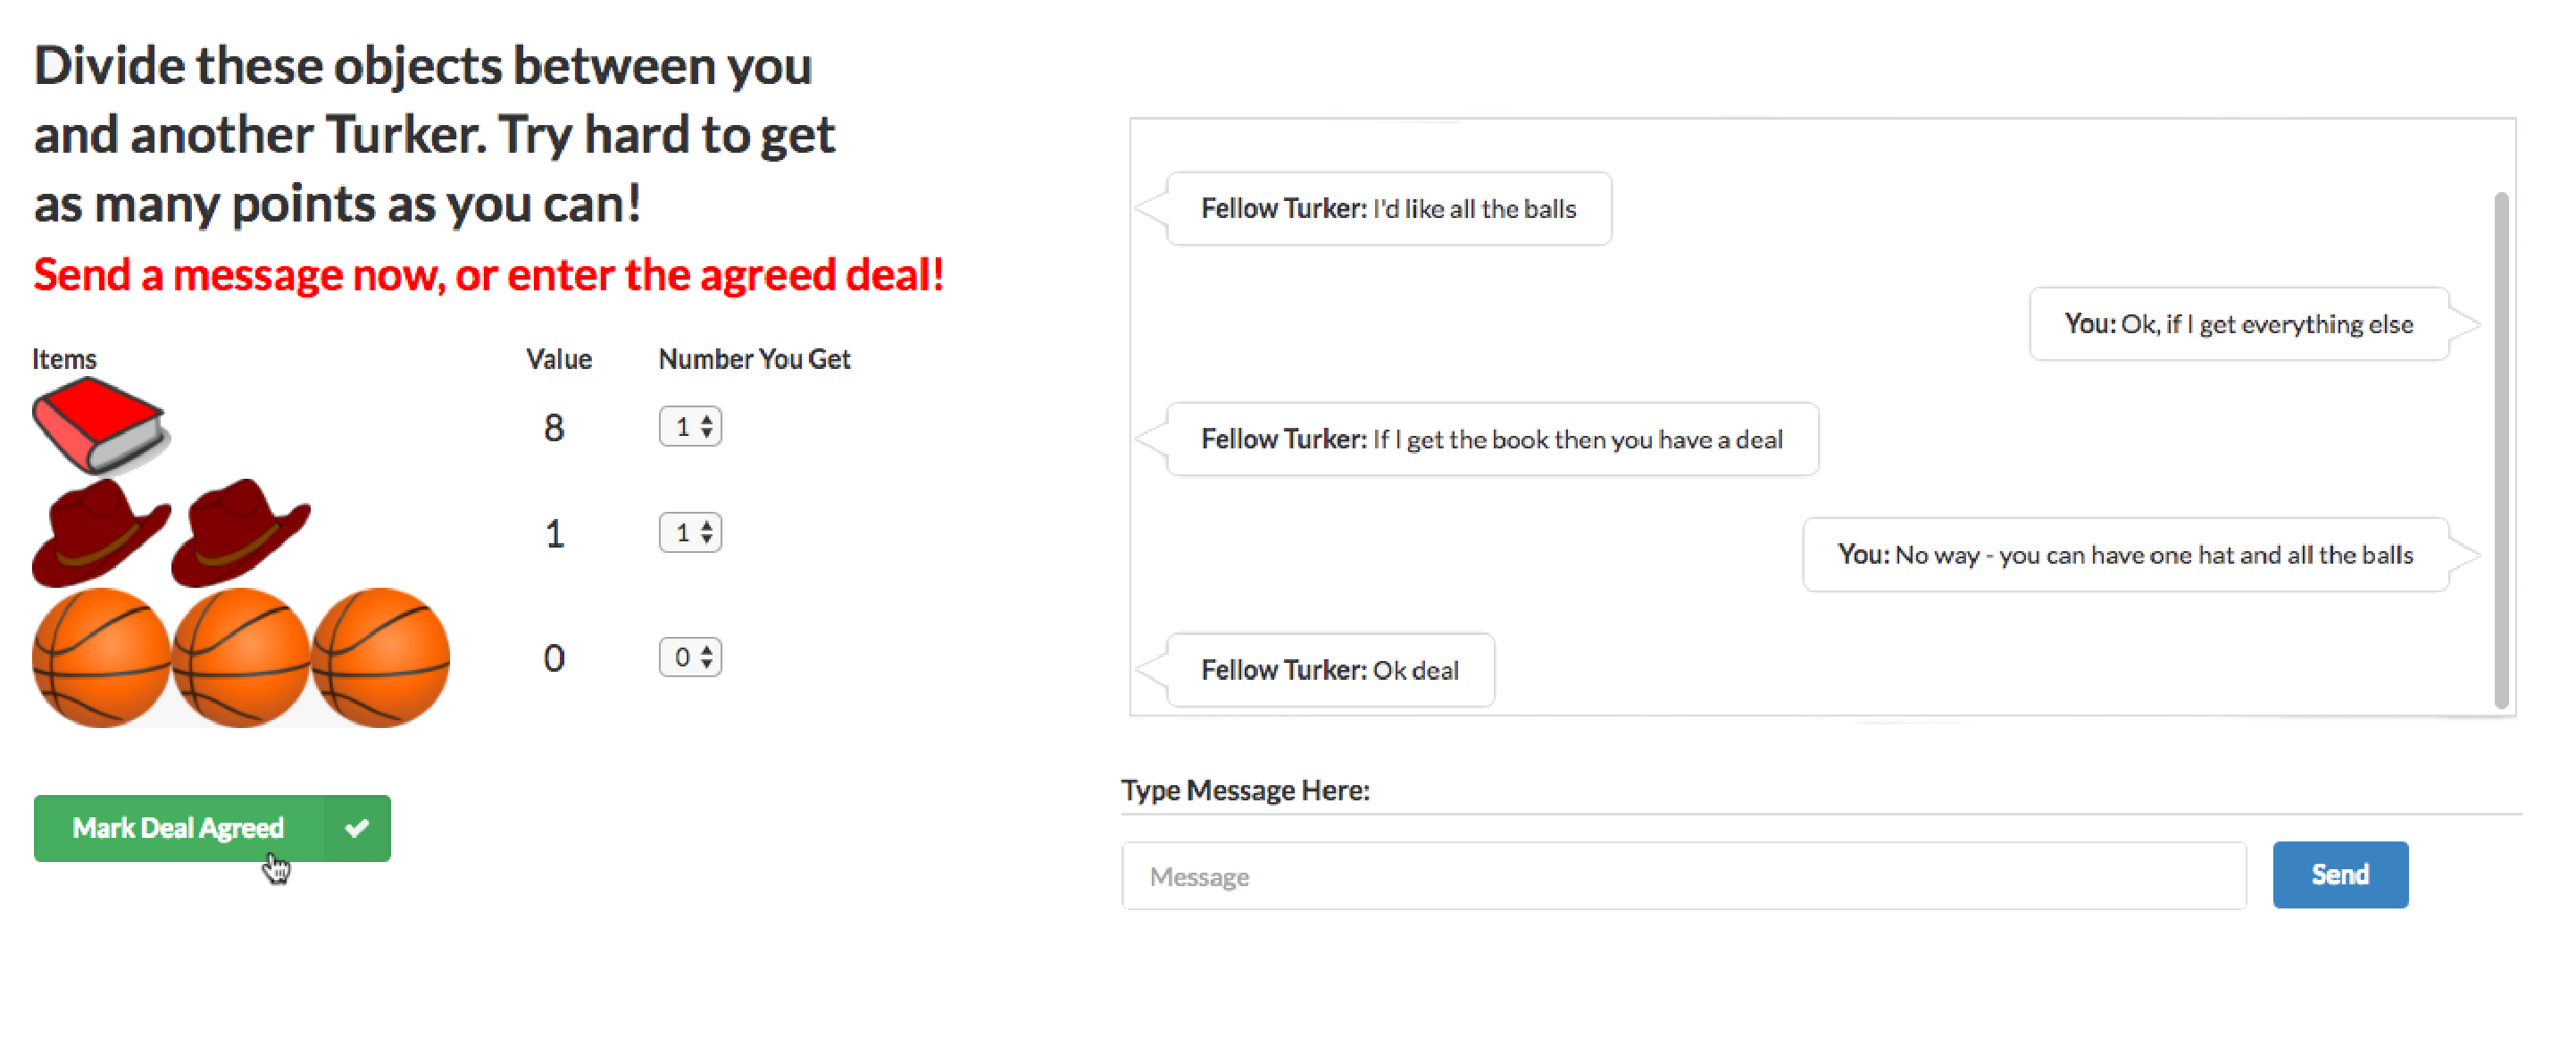
\includegraphics[width=\textwidth]{example_negotiation.eps}
  \vspace{-4.0em}
\caption{\label{figure:turk}谈判对话采集界面,FAIR用其收集\quotes{人-人}谈判文本数据集}
\end{figure*}
FAIR在\citet{DasKottur-6}的基础上建立谈判数据采集界面。
如图\ref{figure:turk}所示,在进行数据采集时,界面会显示各项目的数量、价值、输出\wordnote{
    Output,即输出,表示代理经过对话后认为自己应该取得的各项目数量。
}和对话。
其中,书、帽子和球的数量以Items下的图标数量表示,价值以Values下的数值表示,
输出以Number You Get下的数值表示,对话以对话框形式表述和记录。
以图\ref{figure:turk}为例,项目的数量分别为1、2和3,
价值分别为8、1和0,输出分别为1、1和0,对话记录如对话框所示。